\documentclass[10pt,letter]{article}
	% basic article document class
	% use percent signs to make comments to yourself -- they will not show up.
\usepackage{amsmath}
\usepackage{amssymb}
	% packages that allow mathematical formatting
\usepackage{graphicx}
	% package that allows you to include graphics
\usepackage{setspace}
	% package that allows you to change spacing
\onehalfspacing
	% text become 1.5 spaced
\usepackage{fullpage}
	% package that specifies normal margins

\usepackage{hyperref}
\hypersetup{
    colorlinks=true,
    linkcolor=blue,
    filecolor=magenta,      
    urlcolor=cyan,
}
\urlstyle{same}
\usepackage{siunitx}
\sisetup{output-exponent-marker=\ensuremath{\mathrm{e}}}
\usepackage{float}
\usepackage[autostyle, english=american]{csquotes} \MakeOuterQuote{"} %This line brought to you by Travis
\usepackage{subfig}
\usepackage{pdflscape}
\usepackage{algorithm}
\usepackage[noend]{algpseudocode}

\newcommand{\pluseq}{\mathrel{+}=}
\newcommand{\minuseq}{\mathrel{-}=}

\bibliographystyle{elsarticle-num}

\begin{document}
	% line of code telling latex that your document is beginning


\title{22.212 MOC Homework}

\author{Isaac Meyer\\
        Professor Forget}

	% Note: when you omit this command, the current dateis automatically included
 
\maketitle 
	% tells latex to follow your header (e.g., title, author) commands.

\section*{Overview}
A 2D pseudo-random ray method of characteristics code ("MIMOSA") utilizing constructive solid geometry is developed in python and some performance metrics are analyzed. The code for this project is available at \url{https://github.com/icmeyer/mimosa}. The guideline for the physics protion of the code is mostly guided by John Tramm's work on true random ray method of characteristics \cite{tramm_2017} and OpenMOC \cite{boyd_2014}.

\section*{Method of Characteristics}
The method of characteristics relies on tracking the angular flux of a problem and making a contribution to flat source regions (FSRs). We can calculate this change in $\psi$ with an entry point $s$ and exit $s'$ by  
\[\Psi _ { k g } \left( s ^ { \prime  } \right) = \Psi _ { k , g } \left( s \right) e ^ { - \tau _ { k i g } } + \frac { Q _ { i g } } { \Sigma _ { i g } ^ { T } } \left( 1 - e ^ { - \tau _ { k i g } } \right)\text{ where } \tau_{kig} = \Sigma_{ig}^T(s'-s)\]

\section{Code Description}
Traditional method of characteristics codes solve the eigenvalue problem by using a predetermined set of tracks, and performing power iterations with updates to the source by calculating the contributions of each track. This requires a careful placing of the rays and keeping track of a quadrature for adding track contributions in each FSR. True random ray never uses the same ray twice and instead produces new initial points and angles for each step of the power iteration. In this method of "pseudo random ray", an initial set of rays is created using the random method but reused for each iteration. The basic algorithms for the solution are laid out below. In the code itself the algorithms are generally contained as such:

\begin{table}[h]
\begin{center}
\caption{Code Structure} \label{tab:fourfactors}
\begin{tabular}{ |c|c|c|c|c| } 
\hline
Algorithm & Corresponding File\\ 
\hline
\ref{alg:main} & {main.py} \\
\hline
\ref{alg:tracks} &{ray.py} \\
\hline
\ref{alg:qcalc} & {physics.py} \\
\hline
\ref{alg:transport} & {physics.py} \\
\hline
\end{tabular}
\end{center}
\end{table}

\begin{algorithm}
    \caption{Power Iteration Driver}\label{alg:main}
    \begin{algorithmic}[1]
        \State Lay tracks using Algorithm \ref{alg:tracks}
        \State $k \gets $ guess
        \State $\phi \gets $ guess
        \While{not converged}
        \State $q \gets$ Algorithm \ref{alg:qcalc}
        \State update $k$
        \State  $\phi \gets 0$
        \State  Transport Sweep using Algorithm \ref{alg:transport}
        \For{region $i$}
        \For{group $g$}
        \State $\phi_{i,g}\gets \frac{\phi_{i,g}^{\text{transport}}}{\Sigma_{t,i,g} V_{i} D_{i,\text{tracks}}} + 4\pi Q_{r,e}$ \Comment{Where $D_{i, \text{tracks}}$ is the total active track length over the whole problem} 
        \EndFor
        \EndFor
        \EndWhile
    \end{algorithmic}
\end{algorithm}

\begin{algorithm}
    \caption{Track Laying}\label{alg:tracks}
    \begin{algorithmic}[1]
        \For{ray}
        \State $r\gets (\xi_1,\xi_2)$
        \State $\theta \gets (1-2\xi_3)\frac{\pi}{2} $
        \State $\varphi \gets \xi_42\pi $
        \While{$d_{tot} <$ cutoff}\Comment{We have the answer if r is 0}
        \State find nearest surface
        \State calculate distance $d$
        \State $d_{tot} \pluseq d$
        \If{$d_{tot} > d_{active}$}
        \State store segment with $d$ and region information
        \EndIf
        \EndWhile\label{euclidendwhile}
        \EndFor
    \end{algorithmic}
\end{algorithm}

\begin{algorithm}
    \caption{Q Calculation}\label{alg:qcalc}
    \begin{algorithmic}[1]
        \For{region $i$}
        \For{group $g$}
        \State $q_i \gets \frac { 1 } { 4 \pi \Sigma _ { t , i , g } } \left[ S _ { i , g } + \frac { 1 } { k } F _ { i , g } \right]$ \Comment{Where $S$ and $F$ represent the scatter and fission sources respectively}
        \EndFor
        \EndFor
    \end{algorithmic}
\end{algorithm}

\begin{algorithm}
    \caption{Transport Sweep}\label{alg:transport}
    \begin{algorithmic}[1]
        \State Calculate initial source $q$
        \For{ray $r$}
        \State $\psi_{init} \gets q_i$ \Comment{$i$ denotes the region}
        \For{segment $s$}
        \For{group $g$}
        \State $\tau \gets \Sigma_{tig},d_s$
        \State $\Delta \psi \gets (\psi_g-q_{ig})\cdot(1-e^{-\tau}) $
        \If{$d_{tot} > d_{active}$}
        \State $\phi_{ig} \pluseq 4\pi\Delta \psi$
        \EndIf
        \State $\psi \minuseq \Delta \psi$
        \EndFor
        \EndFor
        \EndFor
    \end{algorithmic}
\end{algorithm}

\section*{Application}
Cross sections for a 3.2\% enriched uranium pincell with $R=0.39218$ cm and pitch$=1.26 cm$ were generated using OpenMC with reflective boundary conditions. Both 2- and 10-group cross sections were generated with the following group structure. 
\begin{table}[h]
\begin{center}
\caption{Energy Groups} \label{tab:fourfactors}
\begin{tabular}{ |c|c|c|c|c| } 
\hline
Groups & Bin Boundaries (eV)\\ 
\hline
2 & $0.0, 1000, 20e6$ \\
\hline
10 &$0.0, 0.058, 0.14, 0.28, 0.625, 4.0, 10.0, 40.0, 5530.0, 821e3, 20e6$ \\
\hline
\end{tabular}
\end{center}
\end{table}

Two problems were run: a pincell with two regions and a 3-by-3 lattice of equivalent enrichment pincells with 4 spatial fuel regions. Visualizations of the MOC geometry are generated by plotting individual segments with the color of the region in which they are contained. Figure \ref{fig:random} shows a good examples of the randomly laid tracks. Plots more representative of the full track lay down are also shown. 

\begin{figure}[H]
    \centering
    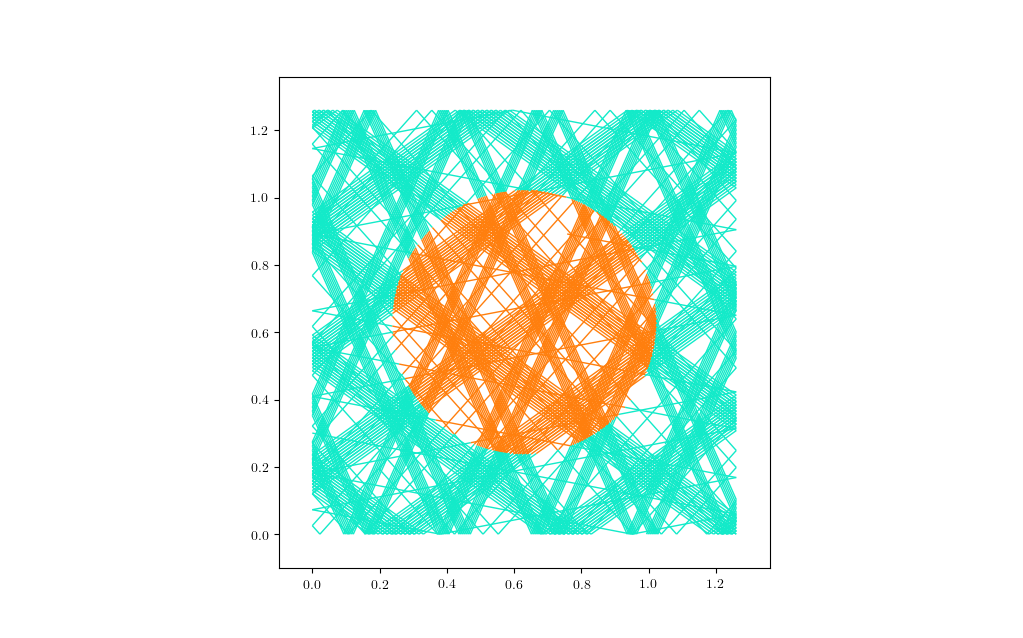
\includegraphics[width=0.8\textwidth]{figs/random_ray.png}
    \caption{Pincell, 4 Rays at 300 cm}
    \label{fig:random}
\end{figure}
\begin{figure}[H]
    \centering
    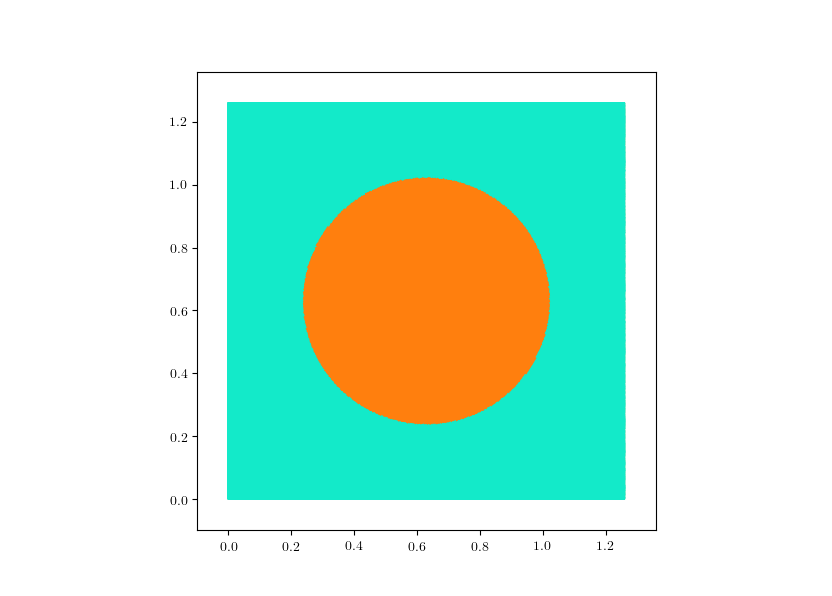
\includegraphics[width=0.8\textwidth]{figs/pincell_geometry.png}
    \caption{Pincell, 1000 Rays at 300 cm}
    \label{fig:5}
\end{figure}
\begin{figure}[H]
    \centering
    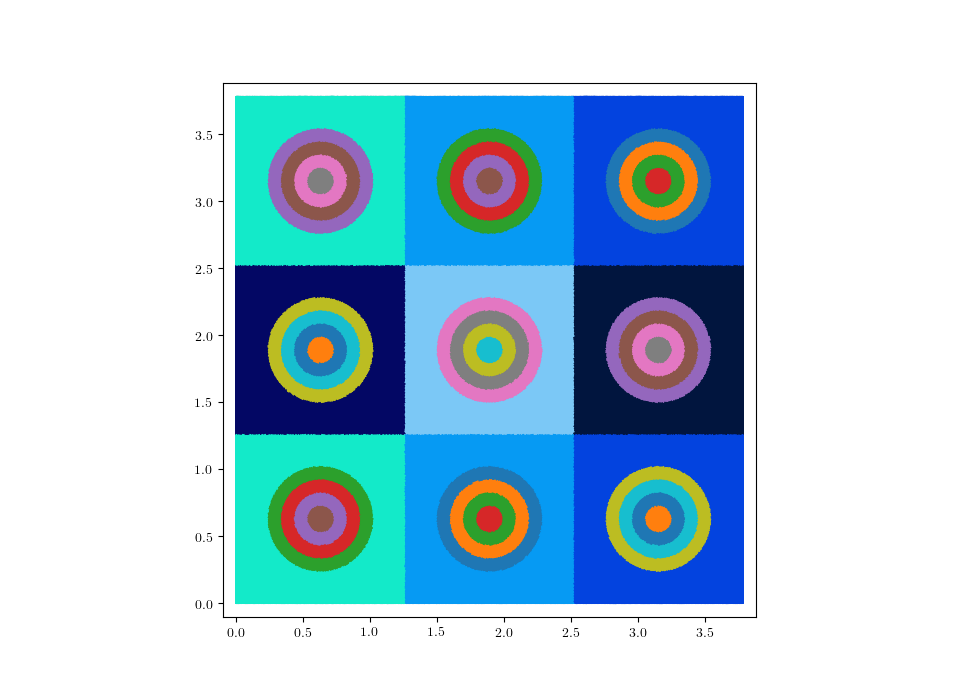
\includegraphics[width=0.8\textwidth]{figs/3by3_geometry.png}
    \caption{3-by-3 with refinement, 1000 Rays at 300 cm}
    \label{fig:5}
\end{figure}

\subsection{Numerical Results}
The simulation convergence criterion was a change in the absolute value of less than $1e-5$. Simulations were run with a total of 1000 rays, ray length of 300 cm and a deadzone of 50 cm. Performance was basedon the wall-clock time of the entire simulation. Results are shown in Table \ref{tab:results}.

\begin{table}[h]
\begin{center}
\caption{Numerical Results} \label{tab:results}
\begin{tabular}{ |c|c|c|c|c| } 
\hline
& Groups & $k_{eff}$ & Performance (Seconds/Segment/Group)\\ 
\hline
OpenMC: pincell & n/a &  1.28941 $\pm$  0.00374  & n/a \\
\hline
MIMOSA: pincell & 2 & 1.28349 & 0.000868\\
\hline
MIMOSA: pincell & 10 & 1.26921 & 0.000144 \\
\hline
MIMOSA: 3-by-3 & 2 &  1.29553 & 0.00189\\
\hline
MIMOSA: 3-by-3 & 10 & 1.27125 & 0.000317\\
\hline
\end{tabular}
\end{center}
\end{table}

\subsection{Behavior of convergence} 
These plots show the behavior of the eigenvalue over the power iterations. 

\begin{figure}[H]
    \centering
    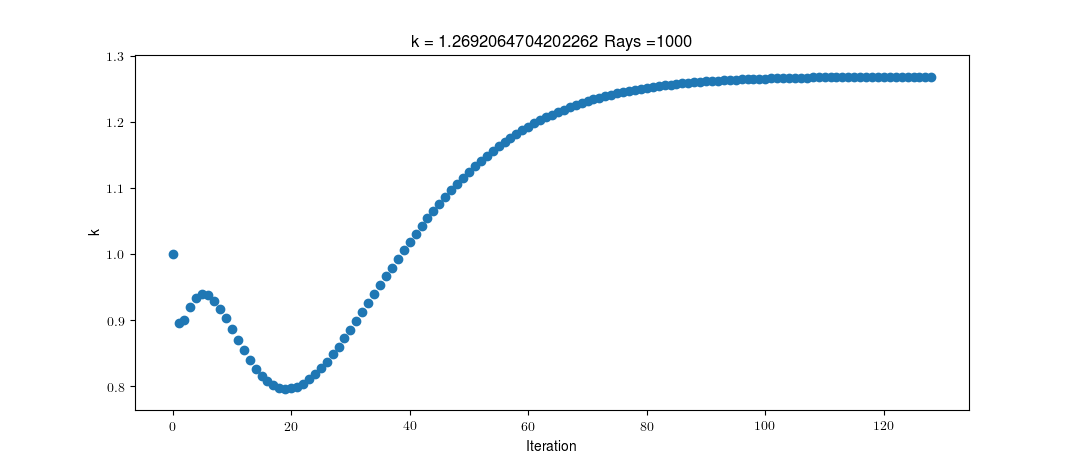
\includegraphics[width=1.05\textwidth]{figs/pincell_ks.png}
    \caption{Pincell}
    \label{fig:5}
\end{figure}
\begin{figure}[H]
    \centering
    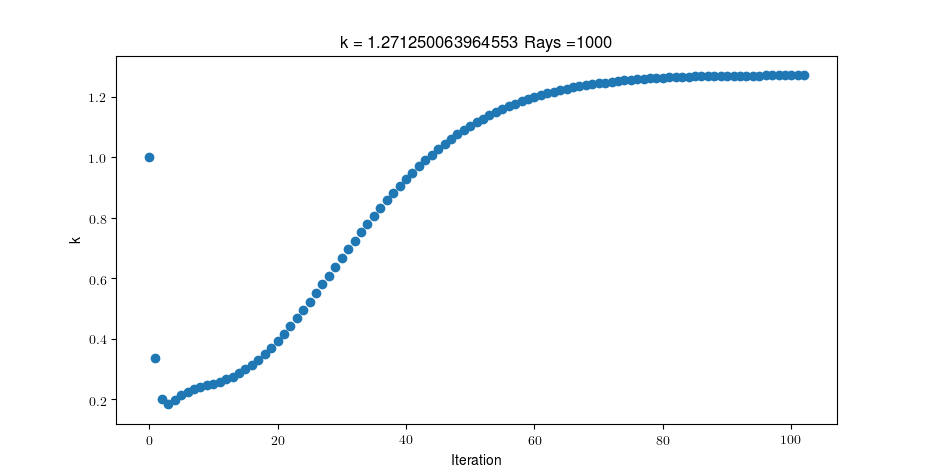
\includegraphics[width=1.05\textwidth]{figs/3by3_ks.png}
    \caption{Pincell}
    \label{fig:5}
\end{figure}
\subsection{Flux} 
The flux results follow what one might expect. The dips at the resonances are clear and while we do not expect a huge difference between moderator and fuel flux, we can see in Figure \ref{fig:flux} that there is a slightly harder spectrum in the fuel as well as larger dips at the resonances. 
\begin{figure}[H]
    \centering
    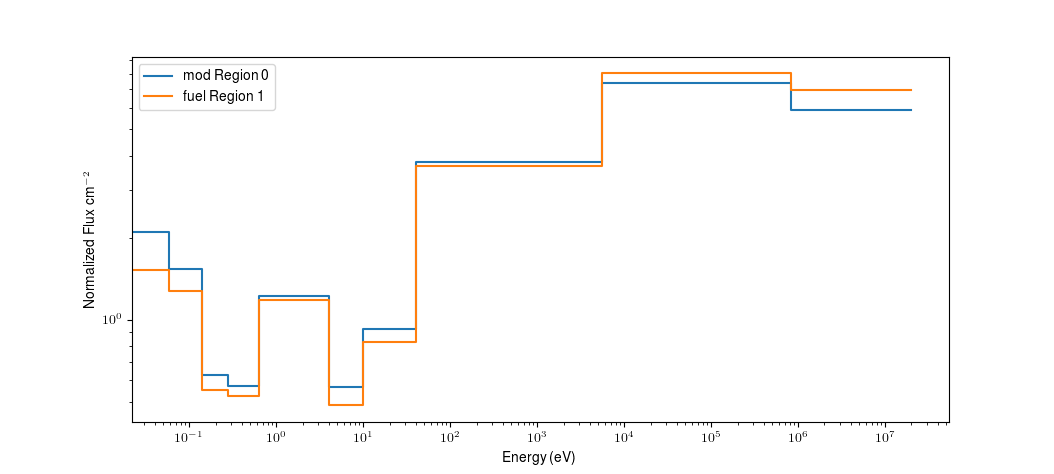
\includegraphics[width=1.05\textwidth]{figs/pincell_flux.png}
    \caption{Pincell 10-group Flux}
    \label{fig:flux}
\end{figure}


\section*{Sensitivity Analysis}
Below are plots of the eigenvalue as a result of changing various parameters. Currently the code does not have the capability to lay a segment partially over a cell which presents a barrier to true sensitivity analysis because currently the tracklength and deadzone must be discretely varying parameters. 

\begin{figure}[H]
    \centering
    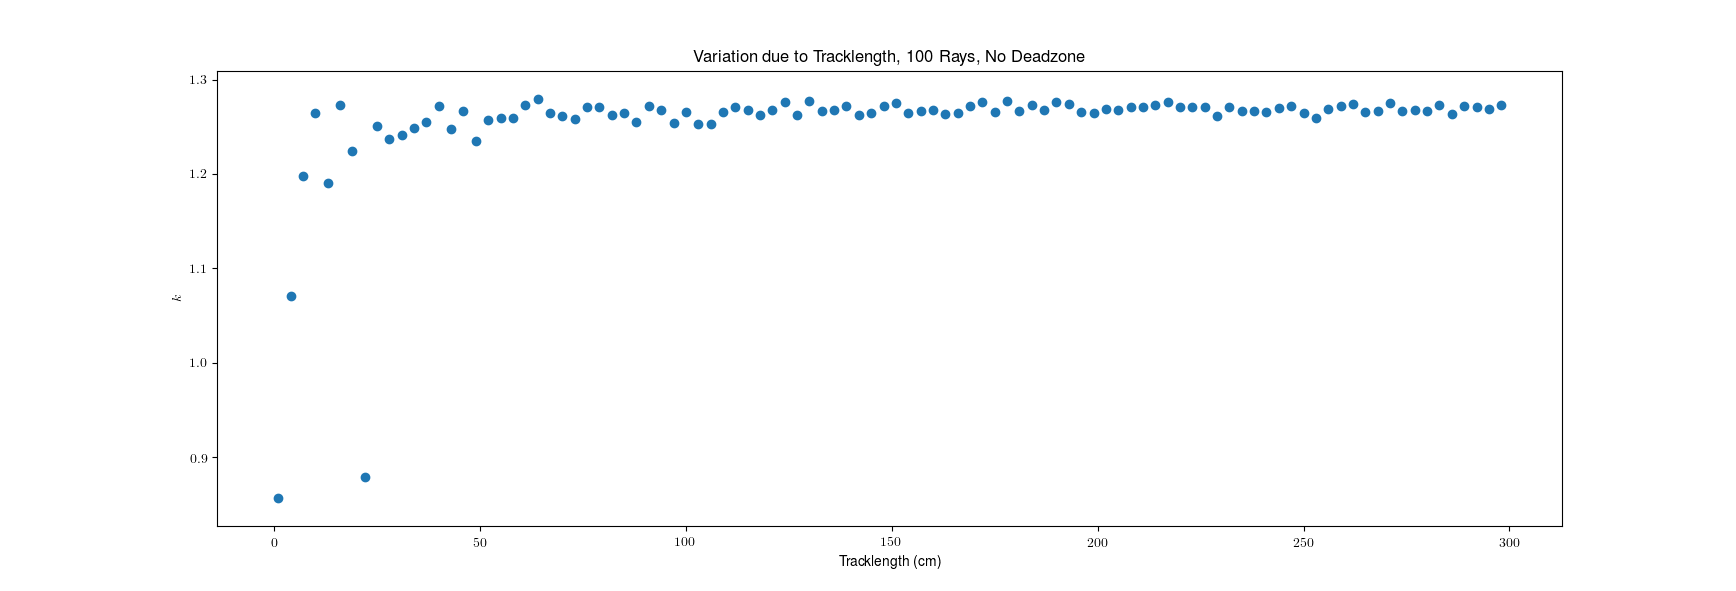
\includegraphics[width=1.2\textwidth]{figs/sensitivity_length1.png}
    \caption{Tracklength}
    \label{fig:5}
\end{figure}
\begin{figure}[H]
    \centering
    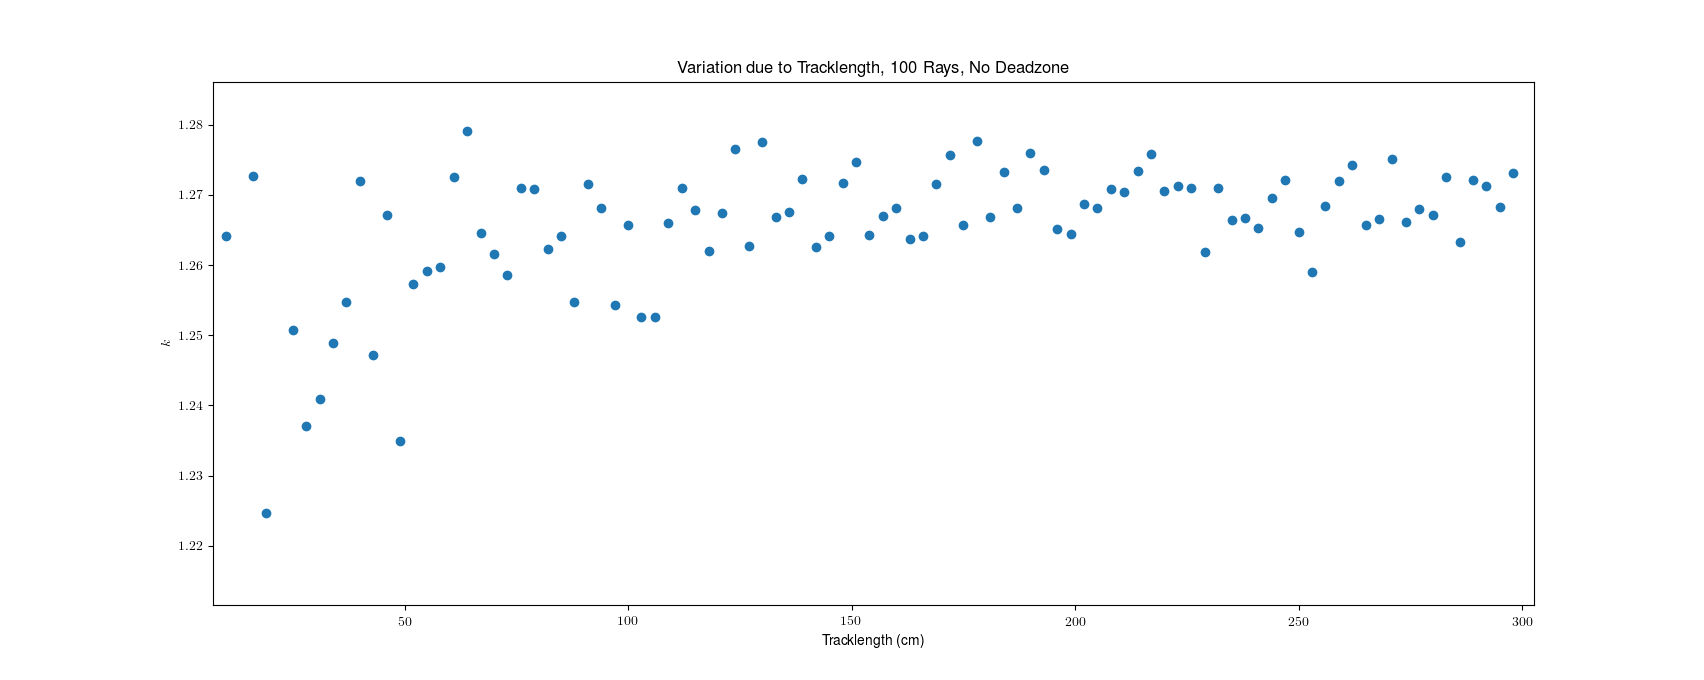
\includegraphics[width=1.2\textwidth]{figs/sensitivity_length2.png}
    \caption{Tracklength}
    \label{fig:5}
\end{figure}
\begin{figure}[H]
    \centering
    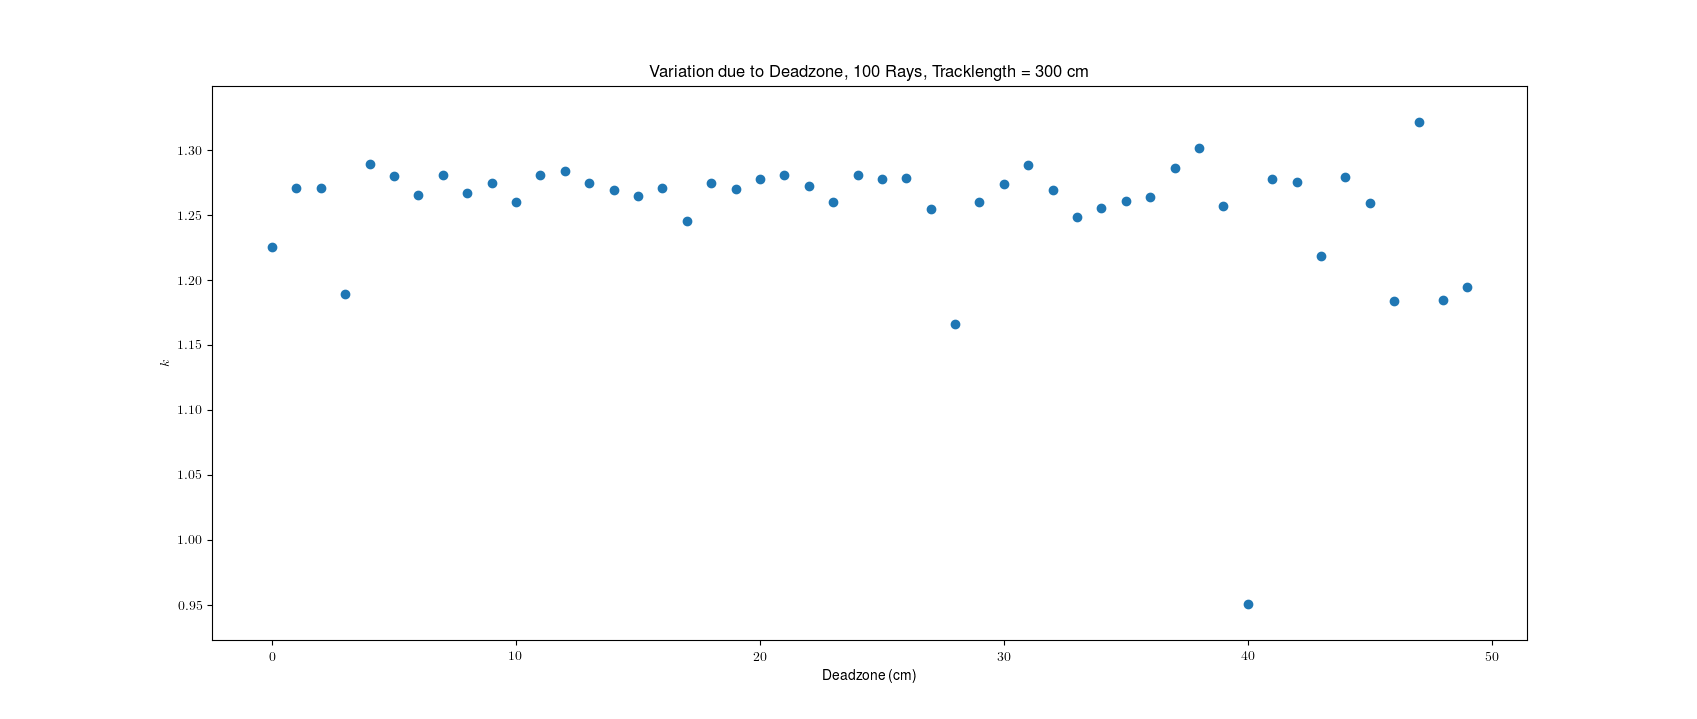
\includegraphics[width=1.2\textwidth]{figs/sensitivity_dz.png}
    \caption{Deadzone}
    \label{fig:5}
\end{figure}
\begin{figure}[H]
    \centering
    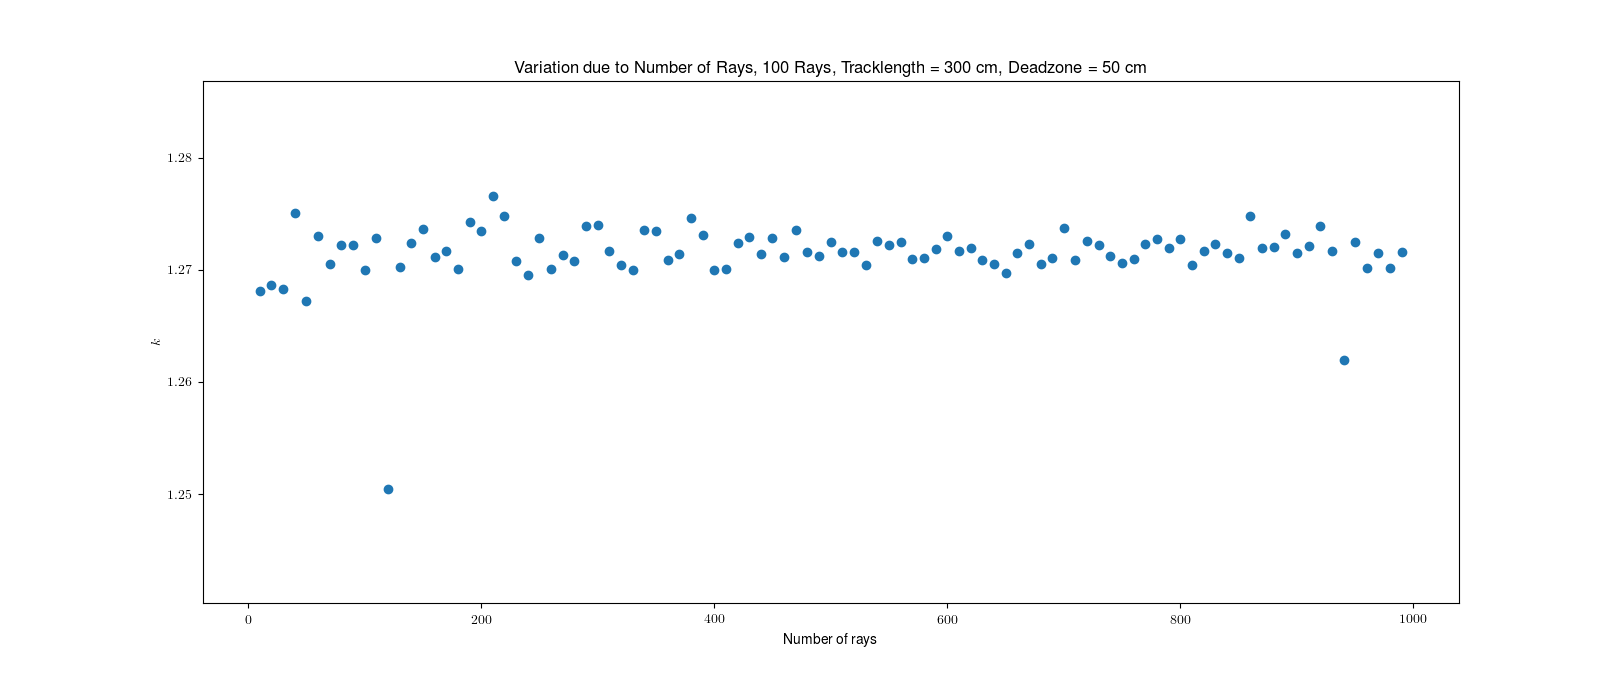
\includegraphics[width=1.2\textwidth]{figs/sensitivity_nrays.png}
    \caption{Number of Rays}
    \label{fig:5}
\end{figure}

At the codes current state this results are not quite expected. While changing the number of rays seems to generally converge the value, the sensitivity to dead zone and tracklength do not follow expected behavior. As stated before, this may be because currently the track placement only adds segments that fully traverse a region. This may introduce some bias in the sampling length of the material. Another issue may be that 100 rays is not enough to accurately capture the angullar dependence of the problem. 

\section*{Note on performance}
The main goal of this initial code was to produce a physical result. There are many aspects that could be improved in performance such as changing which operations need to be done inside of loops, more intelligent surfaces for ray tracing, and porting parts of the code to faster languages. 

\bibliography{bibliography.bib}
\end{document}
	% line of code telling latex that your document is ending. If you leave this out, you'll get an error


% Examples below

% Figure example
% \begin{figure}[H]
%     \centering
%     \includegraphics[width=1.05\textwidth]{figs/Figure_1-5.png}
%     \caption{Problem 5}
%     \label{fig:5}
% \end{figure}

% Equations (simple):
% \[  ]\


% Table Example
% \begin{table}[h]
% \begin{center}
% \caption{Numerical Results} \label{tab:fourfactors}
% \begin{tabular}{ |c|c|c|c|c| } 
% \hline
%  & $k_{eff}$ & Peak Fission Source Value & Location of Peak from center [cm] & Iterations\\ 
% \hline
% Problem 1 & 0.9546 & 1.5442 & 0.0 & 166 \\
% \hline
% Problem 2 & 1.1202 & 1.4627 & 0.0 & 137 \\
% \hline
% Problem 3 & 1.1202 & 1.4605 & 0.0 & 137 \\
% \hline
% Problem 4 & 0.9784 & 1.4329 & 112.0 & 166 \\
% \hline
% Problem 5 & 0.9733 & 1.1124 & 0.0 & 138 \\
% \hline
% \end{tabular}
% \end{center}
% \end{table}


% Code Example
% \begin{verbatim}
%     while True:
%         # Calculate new flux by solving H*phi_1=b_0
%         phinew = np.dot(hinv,b)]
%         # Calculate the new k
%         knew = np.sum(np.dot(fmat,phinew))/np.sum(np.dot(fmat,phiold))*kold
%         if (tolerance met?):
%             break
%         kold = knew
%         #Normalization step
%         phiold = normalize(phinew)
%         phioldsum = phinewsum
%         #Calculate the new fission source
%         b = (1/kold)*np.dot(fmat,phiold)
% \end{verbatim}

%Figure Example
% \begin{figure}[H]
%     \centering
%     \includegraphics[width=0.4\textwidth]{figs/base.png}
%     \caption{CASMO BWR Lattice}
%     \label{fig:matrices}
% \end{figure}

%Algorithm Example
% \begin{algorithm}
%     \caption{Euclid’s algorithm}\label{alg:euclid}
%     \begin{algorithmic}[1]
%         \Procedure{Euclid}{$a,b$}\Comment{The g.c.d. of a and b}
%         \State $r\gets a\bmod b$
%         \While{$r\not=0$}\Comment{We have the answer if r is 0}
%         \State $a\gets b$
%         \State $b\gets r$
%         \State $r\gets a\bmod b$
%         \EndWhile\label{euclidendwhile}
%         \State \textbf{return} $b$\Comment{The gcd is b}
%         \EndProcedure
%     \end{algorithmic}
% \end{algorithm}
